\subsubsubsection{Ports - Incoming}

\paragraph{AuthenticationUseCase} \label{AuthenticationUseCase}
\begin{figure}[H]
    \centering
    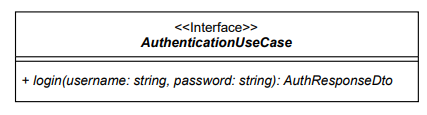
\includegraphics[width=0.95\textwidth]{assets/Backend/authentication_use_case.png}
    \caption{Rappresentazione dell'interfaccia AuthenticationUseCase}
  \end{figure}
\begin{itemize}
    \item \textbf{Descrizione:} questa interfaccia permette di gestire l'autenticazione degli utenti. 
    \item \textbf{Implementazione:} questa interfaccia viene implementata dalla classe \hyperref[AuthenticationService]{(\texttt{AuthenticationService})}. 
    \item \textbf{Metodi:} i metodi dell'interfaccia sono visibili alla classe \hyperref[AuthenticationService]{(\texttt{AuthenticationService})}.
\end{itemize}  

\paragraph{DictionaryUseCase} \label{DictionaryUseCase}
\begin{figure}[H]
    \centering
    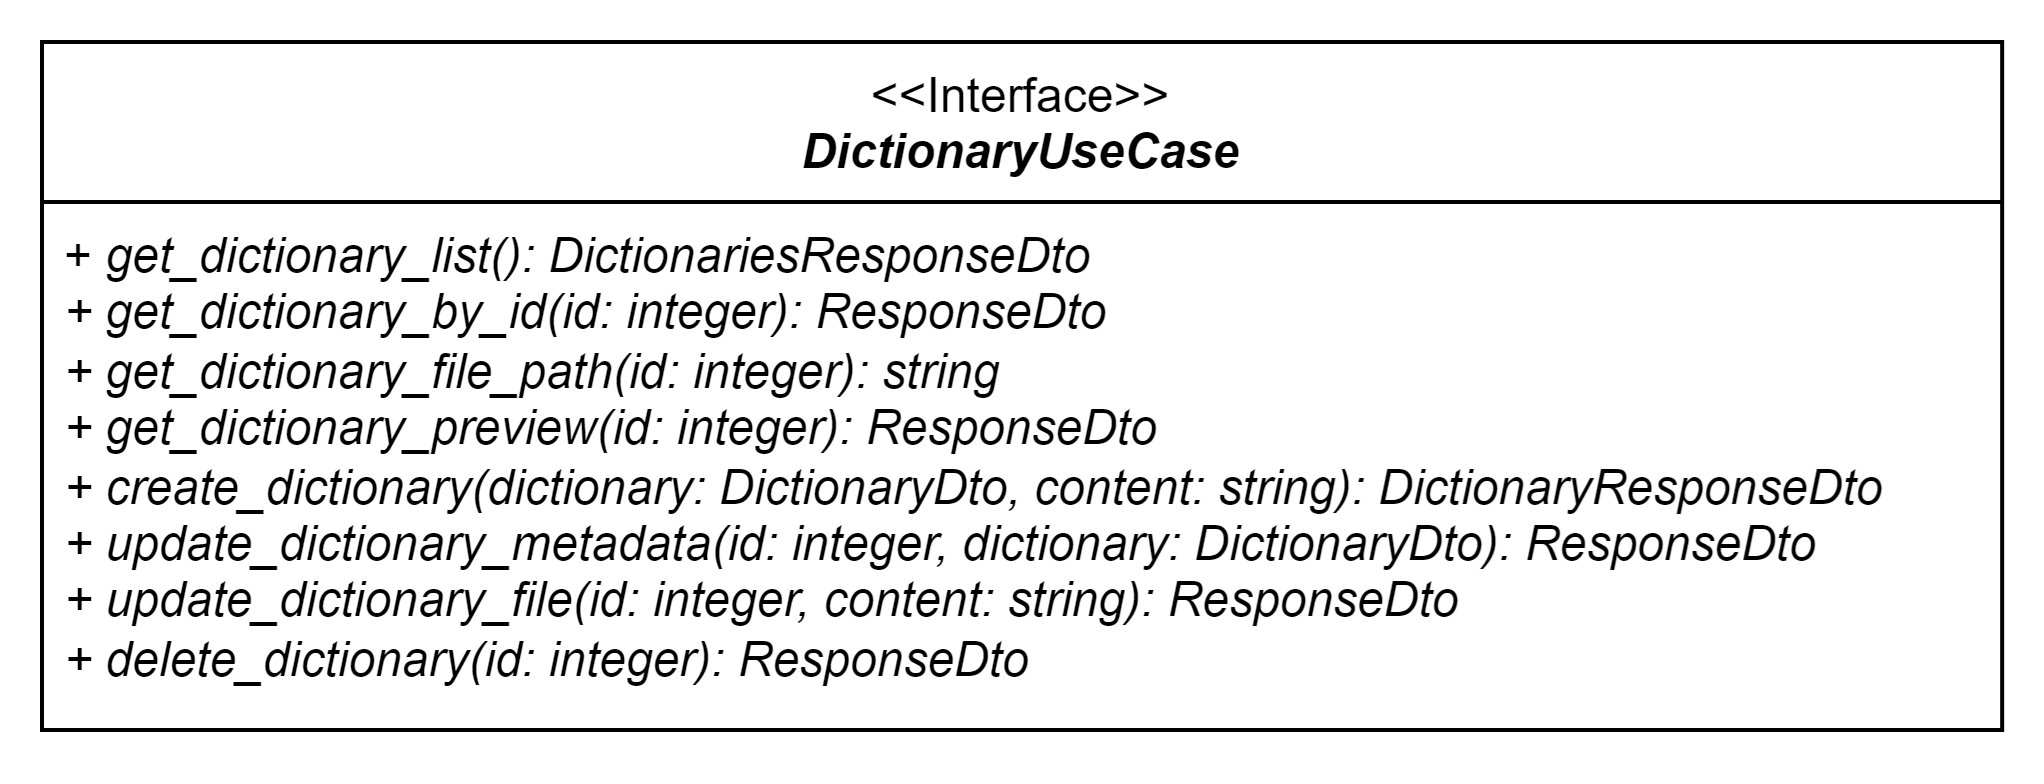
\includegraphics[width=0.95\textwidth]{assets/Backend/dictionary_use_case.png}
    \caption{Rappresentazione dell'interfaccia DictionaryUseCase}
  \end{figure}
\begin{itemize}
    \item \textbf{Descrizione:} questa interfaccia permette di gestire le operazioni sul \glossario{dizionario dati}.
    \item \textbf{Implementazione:} questa interfaccia viene implementata dalla classe \hyperref[DictionaryService]{\texttt{DictionaryService}}.
    \item \textbf{Metodi:} i metodi dell'interfaccia sono visibili alla classe \hyperref[DictionaryService]{(\texttt{DictionaryService})}.
\end{itemize}  

\paragraph{PromptUseCase} \label{PromptUseCase}
\begin{figure}[H]
    \centering
    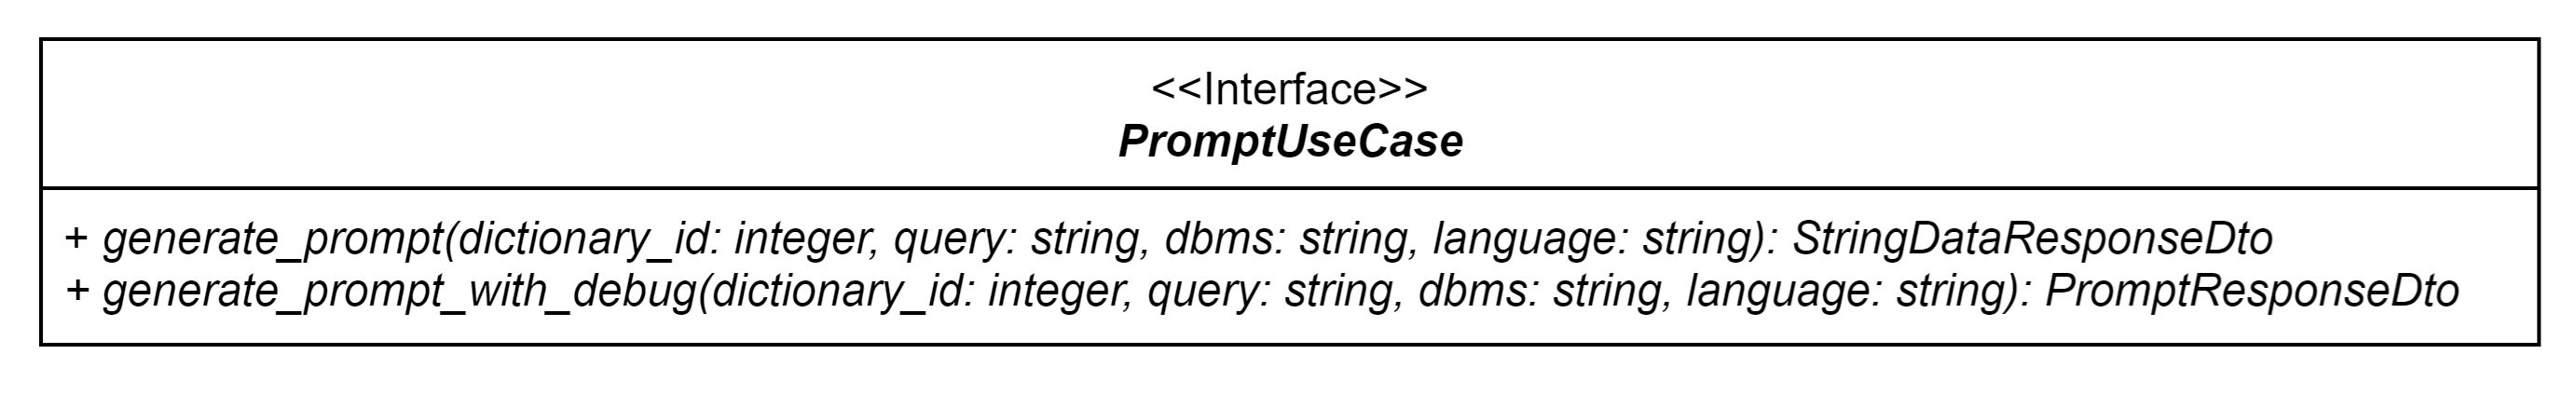
\includegraphics[width=0.95\textwidth]{assets/Backend/prompt_use_case.png}
    \caption{Rappresentazione dell'interfaccia PromptUseCase}
  \end{figure}
\begin{itemize}
    \item \textbf{Descrizione:} questa interfaccia si occupa di gestire le operazioni per la generazione dei \glossario{prompt}.
    \item \textbf{Implementazione:} questa interfaccia viene implementata dalla classe \hyperref[PromptManagementService]{(\texttt{PromptManagementService})}.
    \item \textbf{Metodi:} i metodi dell'interfaccia sono visibili alla classe \hyperref[PromptManagementService]{(\texttt{PromptManagementService})}.
\end{itemize}  

\paragraph{SchemaValidatorUseCase} \label{SchemaValidatorUseCase}
\begin{figure}[H]
    \centering
    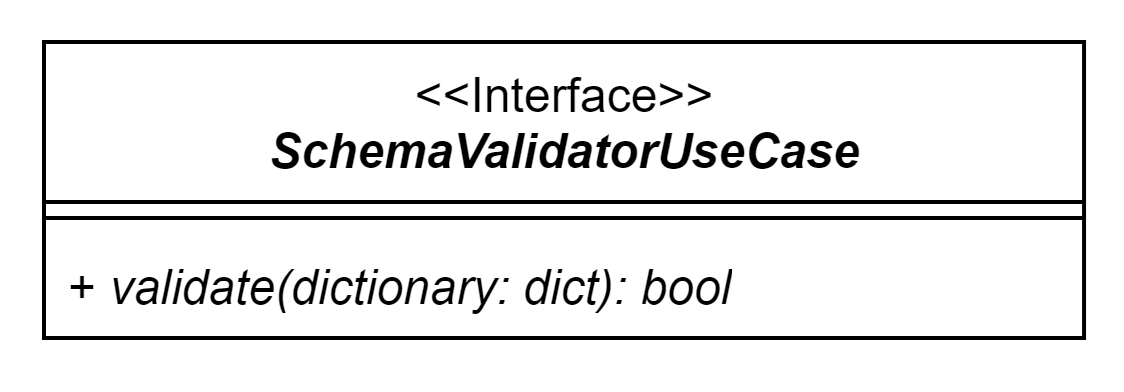
\includegraphics[width=0.95\textwidth]{assets/Backend/schema_validator_use_case.png}
    \caption{Rappresentazione dell'interfaccia SchemaValidatorUseCase}
  \end{figure}
\begin{itemize}
    \item \textbf{Descrizione:} questa interfaccia si occupa della validazione dei \glossario{dizionari dati}.
    \item \textbf{Implementazione:} questa interfaccia viene implementata dalla classe \hyperref[JsonSchemaValidatorAdapter]{(\texttt{JsonSchemaValidatorAdapter})}.
    \item \textbf{Metodi:} i metodi dell'interfaccia sono visibili alla classe \hyperref[JsonSchemaValidatorAdapter]{(\texttt{JsonSchemaValidatorAdapter})}.
    \item \textbf{Dipendenze:}
    \begin{itemize}
        \item \texttt{Dictionary}
    \end{itemize}
\end{itemize}  

\subsubsubsection{Ports - Outcoming}

\paragraph{DebugManagerPort} \label{DebugManagerPort}
\begin{figure}[H]
    \centering
    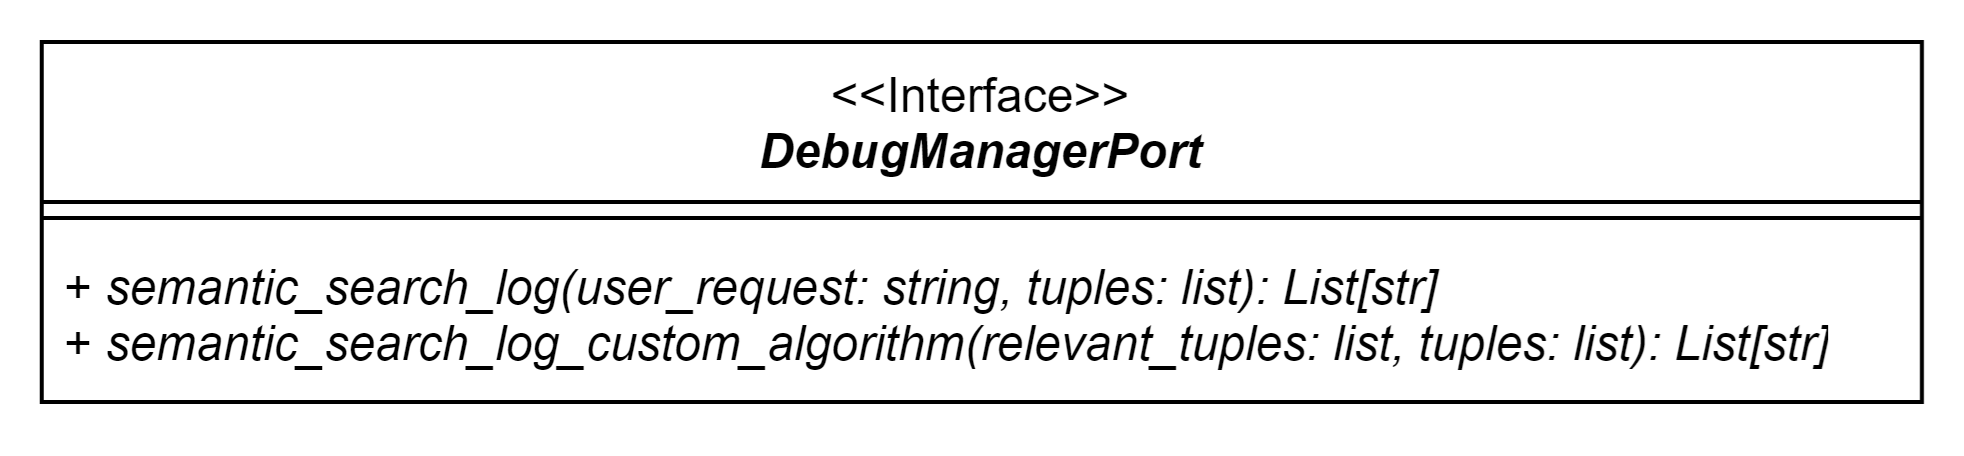
\includegraphics[width=0.95\textwidth]{assets/Backend/debug_manager_port.png}
    \caption{Rappresentazione dell'interfaccia DebugManagerPort}
  \end{figure}
\begin{itemize}
    \item \textbf{Descrizione:} questa interfaccia si occupa della costruzione delle sezioni del documento di \glossario{log} per il \glossario{debug}.
    \item \textbf{Implementazione:} questa interfaccia viene implementata dalla classe \hyperref[TxtaiDebugManagerAdapter]{\texttt{TxtaiDebugManagerAdapter}}.
    \item \textbf{Metodi:} i metodi dell'interfaccia sono visibili alla classe \hyperref[TxtaiDebugManagerAdapter]{\texttt{TxtaiDebugManagerAdapter}}.
\end{itemize}  

\paragraph{EmbeddingsAbstractFactory} \label{EmbeddingsAbstractFactory}
\begin{figure}[H]
    \centering
    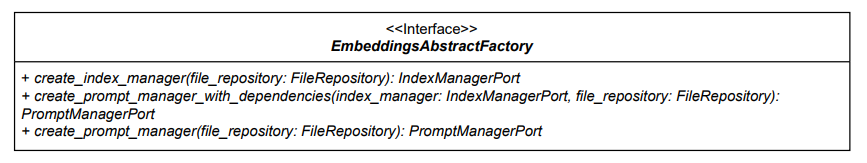
\includegraphics[width=0.95\textwidth]{assets/Backend/embeddings_abstract_factory.png}
    \caption{Rappresentazione dell'interfaccia EmbeddingsAbstractFactory}
  \end{figure}
\begin{itemize}
    \item \textbf{Descrizione:} questa interfaccia si occupa della creazione dell'index manager e delle classi per la gestione dei \glossario{prompt}.
    \item \textbf{Implementazione:} questa interfaccia viene implementata dalla classe \hyperref[TxtaiEmbeddingsManagerFactory]{\texttt{TxtaiEmbeddingsManagerFactory}}.
    \item \textbf{Metodi:} i metodi dell'interfaccia sono visibili alla classe \hyperref[TxtaiEmbeddingsManagerFactory]{\texttt{TxtaiEmbeddingsManagerFactory}}.
    \item \textbf{Dipendenze:}
    \begin{itemize}
        \item \texttt{DebugManagerPort};
        \item \texttt{IndexManagerPort};
        \item \texttt{PromptManagerPort};
    \end{itemize}
\end{itemize}  

\paragraph{IndexManagerPort} \label{IndexManagerPort}
\begin{figure}[H]
    \centering
    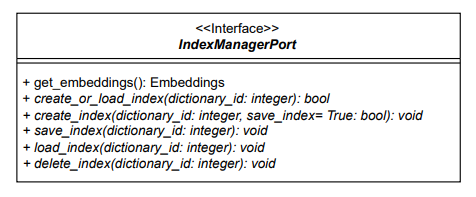
\includegraphics[width=0.95\textwidth]{assets/Backend/index_manager_port.png}
    \caption{Rappresentazione dell'interfaccia IndexManagerPort}
  \end{figure}
\begin{itemize}
    \item \textbf{Descrizione:} questa interfaccia si occupa delle operazioni CRUD per gli indici degli embeddings.
    \item \textbf{Implementazione:} questa interfaccia viene implementata dalla classe \hyperref[TxtaiIndexManagerAdapter]{\texttt{TxtaiIndexManagerAdapter}}.
    \item \textbf{Metodi:} i metodi dell'interfaccia sono visibili alla classe \hyperref[TxtaiIndexManagerAdapter]{\texttt{TxtaiIndexManagerAdapter}}.
\end{itemize} 

\paragraph{PromptManagerPort} \label{PromptManagerPort}
\begin{figure}[H]
    \centering
    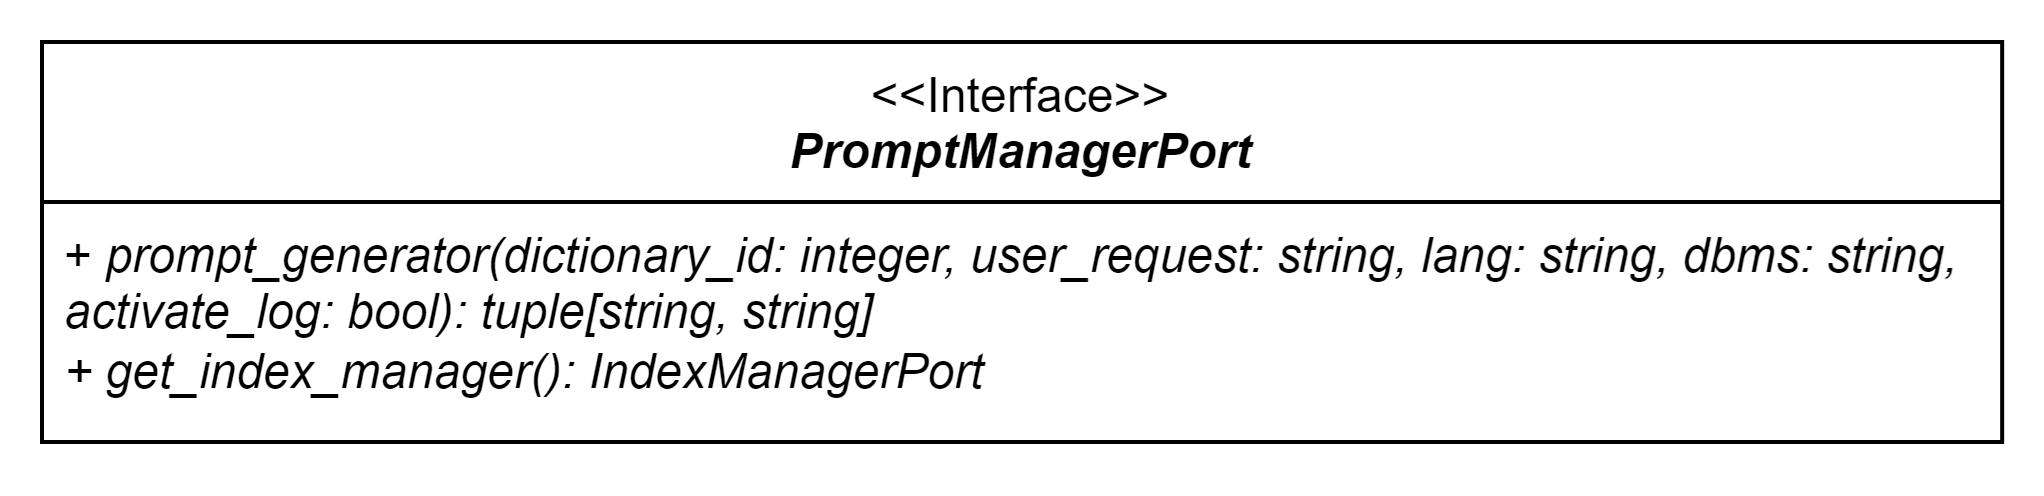
\includegraphics[width=0.95\textwidth]{assets/Backend/prompt_manager_port.png}
    \caption{Rappresentazione dell'interfaccia PromptManagerPort}
  \end{figure}
\begin{itemize}
    \item \textbf{Descrizione:} questa interfaccia si occupa del recupero delle informazioni e la generazione del prompt.
    \item \textbf{Implementazione:} questa interfaccia viene implementata dalla classe \hyperref[TxtaiPromptManagerAdapter]{\texttt{TxtaiPromptManagerAdapter}}. 
    \item \textbf{Attributi:} FIXME (ci sono degli attributi, ma è un'interfaccia)
    \item \textbf{Metodi:} i metodi dell'interfaccia sono visibili alla classe \hyperref[TxtaiPromptManagerAdapter]{\texttt{TxtaiPromptManagerAdapter}}.
    \item \textbf{Dipendenze:}
    \begin{itemize}
        \item \texttt{IndexManagerPort};
        \item \texttt{DebugManagerPort}.
    \end{itemize}
\end{itemize} 

\paragraph{AuthenticationRepository} \label{AuthenticationRepository}
\begin{figure}[H]
    \centering
    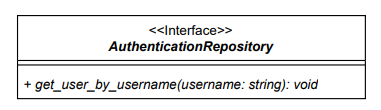
\includegraphics[width=0.95\textwidth]{assets/Backend/authentication_repository.png}
    \caption{Rappresentazione dell'interfaccia AuthenticationRepository}
  \end{figure}
\begin{itemize}
    \item \textbf{Descrizione:} questa interfaccia si occupa del recupero degli utenti.
    \item \textbf{Implementazione:} questa interfaccia viene implementata dalla classe \hyperref[SqlAlchemyAuthenticationRepositoryAdapter]{\texttt{SqlAlchemyAuthenticationRepositoryAdapter}}.
    \item \textbf{Metodi:} i metodi dell'interfaccia sono visibili alla classe \hyperref[SqlAlchemyAuthenticationRepositoryAdapter]{\texttt{SqlAlchemyAuthenticationRepositoryAdapter}}.
\end{itemize} 

\paragraph{DbManagerAbstractFactory} \label{DbManagerAbstractFactory}
\begin{figure}[H]
    \centering
    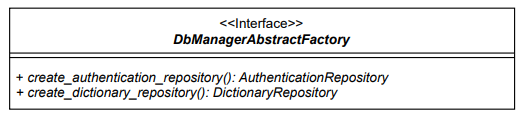
\includegraphics[width=0.95\textwidth]{assets/Backend/db_manager_abstract_factory.png}
    \caption{Rappresentazione dell'interfaccia DbManagerAbstractFactory}
  \end{figure}
\begin{itemize}
    \item \textbf{Descrizione:} questa interfaccia si occupa della creazione di istanze delle classi \texttt{AuthenticationRepository} e \texttt{DictionaryRepository}.
    \item \textbf{Implementazione:} questa interfaccia viene implementata dalla classe \hyperref[SqlAlchemyDbManagerFactory]{\texttt{SqlAlchemyDbManagerFactory}}.
    \item \textbf{Metodi:} i metodi dell'interfaccia sono visibili alla classe \hyperref[SqlAlchemyDbManagerFactory]{\texttt{SqlAlchemyDbManagerFactory}}.
    \item \textbf{Dipendenze:}
    \begin{itemize}
        \item \texttt{AuthenticationRepository};
        \item \texttt{DictionaryRepository}.
    \end{itemize}
\end{itemize} 

\paragraph{DictionaryRepository} \label{DictionaryRepository}
\begin{figure}[H]
    \centering
    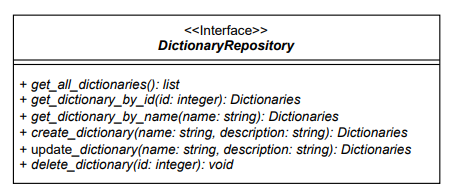
\includegraphics[width=0.95\textwidth]{assets/Backend/dictionary_repository.png}
    \caption{Rappresentazione dell'interfaccia DictionaryRepository}
  \end{figure}
\begin{itemize}
    \item \textbf{Descrizione:} questa interfaccia si occupa del recupero dei dizionari dati e delle operazioni CRUD su questi.
    \item \textbf{Implementazione:} questa interfaccia viene implementata dalla classe \hyperref[SqlAlchemyDictionaryRepositoryAdapter]{\texttt{SqlAlchemyDictionaryRepositoryAdapter}}.
    \item \textbf{Metodi:} i metodi dell'interfaccia sono visibili alla classe \hyperref[SqlAlchemyDictionaryRepositoryAdapter]{\texttt{SqlAlchemyDictionaryRepositoryAdapter}}.
\end{itemize} 

\paragraph{FileRepository} \label{FileRepository}
\begin{figure}[H]
    \centering
    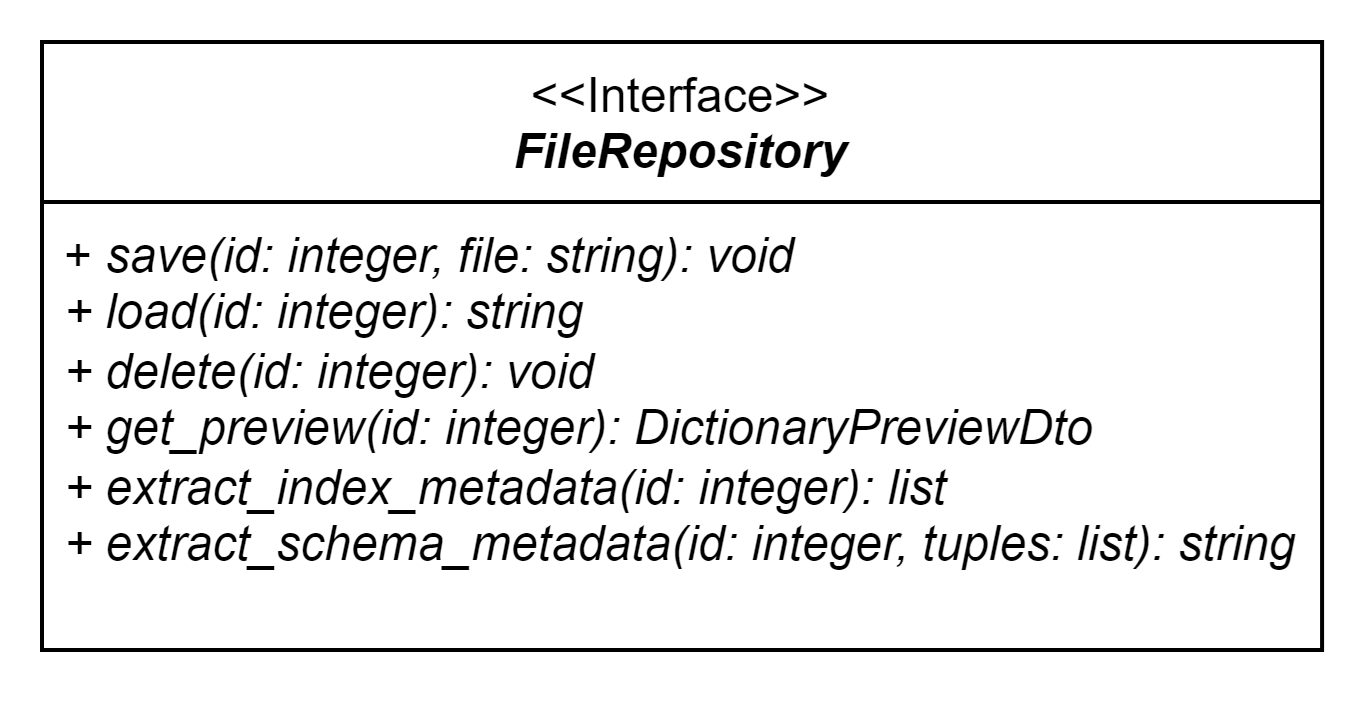
\includegraphics[width=0.95\textwidth]{assets/Backend/file_repository.png}
    \caption{Rappresentazione dell'interfaccia FileRepository}
  \end{figure}
\begin{itemize}
    \item \textbf{Descrizione:} questa interfaccia si occupa delle operazioni CRUD sui file dei dizionari dati.
    \item \textbf{Implementazione:} questa interfaccia viene implementata dalla classe \hyperref[JsonFileAdapter]{\texttt{JsonFileAdapter}}.
    \item \textbf{Metodi:} i metodi dell'interfaccia sono visibili alla classe \hyperref[JsonFileAdapter]{\texttt{JsonFileAdapter}}.
\end{itemize} 